% Author: Izaak Neutelings (Februari, 2020)
\documentclass[border=3pt,tikz]{standalone}
\usepackage{amsmath} % for \dfrac
\usepackage{physics,siunitx}
%\usepackage{tikz,pgfplots}
\tikzset{>=latex} % for LaTeX arrow head
\usetikzlibrary{calc}
\usepackage{xcolor}
\colorlet{myblue}{blue!70!black}
\colorlet{myred}{red!70!black}
\tikzstyle{bline}=[myblue,thick]
\tikzstyle{rline}=[myred,thick]
\def\xmax{6}
\def\ymax{4}
\def\tick#1#2{\draw[thick] (#1) ++ (#2:0.025*\ymax) --++ (#2-180:0.05*\ymax)}
\newcommand\tauh{\tau_\mathrm{h}}
\newcommand\pt{p_\mathrm{T}}

\begin{document}



% TAU ENERGY SCALE UNCERTAINTY
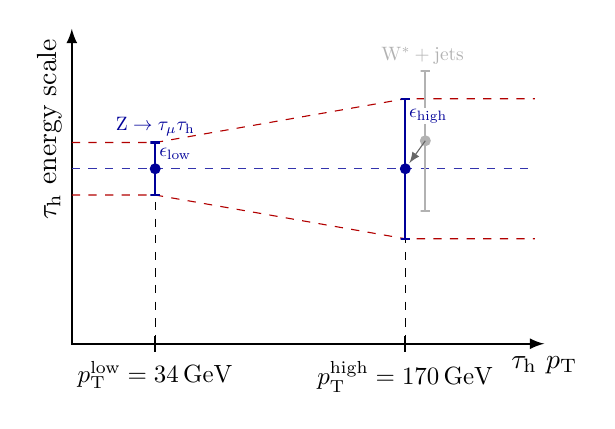
\begin{tikzpicture}
  \def\tes{     1.0*\ymax/1.8}
  \def\unclow{ 0.15*\ymax/1.8}
  \def\unchigh{0.40*\ymax/1.8}
  \def\ptlow{  30.0*\xmax/170}
  \def\pthigh{120.0*\xmax/170}
  \def\bar{    0.01*\xmax}
  \coordinate (O) at (0,0);
  \coordinate (X) at (\xmax,0);
  \coordinate (Y) at (0,\ymax);
  \coordinate (T) at (0,\tes);
  \coordinate (TL) at (\ptlow,\tes);
  \coordinate (TH) at (\pthigh,\tes);
  \coordinate (TW) at (1.06*\pthigh,1.16*\tes);
  \coordinate (TF) at (0.98*\xmax,\tes);
  \coordinate (PL) at (\ptlow,0);
  \coordinate (PH) at (\pthigh,0);
  %\path let \p{TL}=(TL) in coordinate (PL) at (\x{TL},0);
  %\path let \p{TH}=(TH) in coordinate (PH) at (\x{TH},0);
  \def\point#1#2#3{ %#4{
    \draw[thick,#3] (#1) --++ (0,-#2) coordinate (#1low)
              (#1) --++ (0,#2) coordinate (#1high); % node[midway,right=-1,scale=0.9] {#4};
    \draw[thick,#3] (#1low)  --++ (-\bar,0) --++ (2*\bar,0);
    \draw[thick,#3] (#1high) --++ (-\bar,0) --++ (2*\bar,0);
    \fill[#3] (#1) circle (0.07);
  }
  
  % AXIS
  \draw[<->,thick]
    (X) node[below=1] {$\tauh$ $\pt$} -- (O) -- (Y) node[rotate=90,above left] {$\tauh$ energy scale};
  %\fill (TL) circle (0.07);
  %\fill (TH) circle (0.07);
  
  % DASHES
  \draw[dashed,blue!60!black!80] (T) -- (TF);
  \draw[dashed] (TL) -- (PL);
  \draw[dashed] (TH) -- (PH);
  \tick{PL}{90} node[below,scale=0.9] {$\pt^\text{low} = \SI{34}{GeV}$};
  \tick{PH}{90} node[below,scale=0.9] {$\pt^\text{high} = \SI{170}{GeV}$};
  \draw[dashed,red!70!black]
    ($(T)+(0,\unclow)$) -- ($(TL)+(0,\unclow)$) -- ($(TH)+(0,\unchigh)$) -- ($(TF)+(0,\unchigh)$);
  \draw[dashed,red!70!black]
    ($(T)-(0,\unclow)$) -- ($(TL)-(0,\unclow)$) -- ($(TH)-(0,\unchigh)$) -- ($(TF)-(0,\unchigh)$);
  
  % POINTS
  \point{TL}{\unclow}{blue!60!black} %{$\epsilon_\text{low}$}
  \point{TH}{\unchigh}{blue!60!black} %{$\epsilon_\text{high}$}
  \point{TW}{\unchigh}{black!30} %{$\epsilon_\text{high}$}
  \node[above,scale=0.7,blue!60!black] at (TLhigh) {$\mathrm{Z} \to \tau_\mu \tauh$};
  \node[left=1,above,scale=0.7,black!30] at (TWhigh) {$\mathrm{W}^*+\text{jets}$};
  \node[left=2,above right=1,scale=0.7,blue!60!black] at (TL) {$\epsilon_\text{low}$};
  \node[right=1,above=6,scale=0.7,blue!60!black,fill=white,inner sep=0.5] at (TW) {$\epsilon_\text{high}$};
  \draw[->,black!60,shorten >=2.5] (TW) -- (TH); %,shorten <=0.5
  
\end{tikzpicture}




\end{document}
